\documentclass[a4paper]{article} 
\usepackage[intlimits,tbtags]{amsmath}
\usepackage{amssymb}   
\usepackage{amsfonts}
\usepackage{latexsym}  
\usepackage{amsxtra}   
\usepackage{amstext}   
\usepackage{bm}        
\usepackage{amsthm}    
\usepackage{amscd}     
\usepackage[dvipsnames]{xcolor}
\usepackage{marvosym}
\usepackage[utf8]{inputenc}
\usepackage[shortlabels]{enumitem}
\usepackage{array}
\usepackage{hyperref}
\usepackage{graphicx}
\usepackage[english]{babel}
\usepackage{amsmath}
\usepackage{graphicx}
\usepackage[colorinlistoftodos]{todonotes}
\newcommand{\E}{\mathbb{E}}
\newcommand{\hatt}{\hat{\theta}_m}
\usepackage{algorithm}
\usepackage{algpseudocode}
\usepackage{tikz}

\title{Summary of the Deep Learning Lecture at the University of Bonn}


\author{Tim Nogga}

\begin{document}


\maketitle
\tableofcontents
                                                                                                                                
\section{Introduction}
\subsection{Task T}
Machine Learning Tasks describes how a machine learning system learns from data. Such data can be images(pixels) among many. Typical Tasks include Klassification, Regression, and Density Function Estimation.

\subsection{Experience E}
Specifies the Information an Algorithm can use during the Learning Process.

\subsubsection{Supervised Learning}
The Algorithm is given a dataset with the correct answers. The Algorithm then tries to learn the mapping from the input to the output. This can be described with an Estimation $p_data(y|x)$.

\subsubsection{Unsupervised Learning}
The Algorithm is given a dataset without the correct answers. The Algorithm then tries to learn the underlying structure of the data. This can be described with an Estimation $p_data(x)$.

\subsection{Performance Measure P}
Learning Algorithms can be evaluated based on their Performance. In Classification Problems, the Accuracy is a common measure. %TODO: what is a mittlere logarithmische Wahrscheinlichkeits von Samples?
The Perfomance Measure is calculated on a Test Set, which is not used during the Training Process. So there a are two sets a Test Set and a Training Set. 

\subsection{Training Error, Test Error and Generalization}
Generalization is the ability of an algorithm to perform well on previously unseen data. During Training the Training Error should be reduced, but the Test Error should be reduced as well. If the Training Error is reduced but the Test Error is not, the algorithm is overfitting. Meaning the algorithm is learning the noise in the data instead of the underlying structure. But if the Test Error is not even reduced the algorithm is underfitting.

\subsection{Capacity}
Overfitting and underfitting are also dependent on the capacity of the model. Say you take a model with with a low capacity, it will underfit the data, as it is not able to learn the underlying structure. But if a model with high Capacity is used, it will just memorize the data and thus overfit, as it is not able to generalize.

\subsection{Capacity vs Error}
\begin{figure}[h]
    \centering
    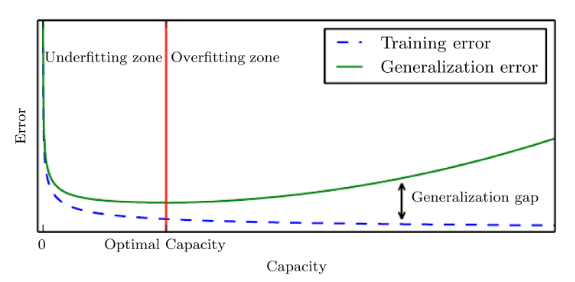
\includegraphics[width=0.8\textwidth]{images/capacity.png}
    \caption{}
    \label{fig:}
\end{figure}
It becomes apparent that the Training Error decreases with increasing Capacity. But the Test Error decreases first and then increases again. This is due to the fact that the model is overfitting the data, thus not able to generalize anymore. This is also why it is called Generalization Gap.

\subsection{Hyperparameters}
Leraning Algorithms usually have Hyperparameters which are paramters not learned during Training, but set before. These could be things such as Model Capacity and Learning Rate. This poses the Question wether Capacity Hyperparameters can be derived from the Trainingset. The answer is no, since the Learning Algorithm would always choose the highest Capacity, as it would always reduce the Training Error.

\subsection{Cross Validation}
Cross Validation can be used to determine the best Hyperparameters. The Training Set is split into k parts. Then the Algorithm is trained on k-1 parts and tested on the remaining part. This is done k times, so that every part is used as a Test Set once. The average Test Error is then used to determine the best Hyperparameters. 

\section{Recap Statistics}
\subsection{Terms and Definitions}
\begin{itemize}
    \item \textbf{Sample Space} $\Omega$: Set of all possible outcomes of an experiment. For example a dice roll has a Sample Space of $\Omega = \{1,2,3,4,5,6\}$
    \item \textbf{Event} $A$: Subset of the Sample Space. For example the Event of rolling an even number is $A = \{2,4,6\}$
    \item \textbf{Sigma Algebra} Collection of Events. For example the Sigma Algebra of the dice roll is $\sigma(\Omega) = \{\emptyset, \{1,2,3,4,5,6\}, \{1,3,5\}, \{2,4,6\}\}$
    \item \textbf{Measurable space} $(\Omega, \mathcal{A})$: Is a Measurable Space if $\Omega$ is a Sample Space and $\mathcal{A}$ is a Sigma Algebra.
\end{itemize}

\begin{itemize}
    \item \textbf{Probability Density Function if $\Omega$ is Discrete} x $p: \Omega \rightarrow [0,1]$ with $\sum_{\omega \in \Omega} p(\omega) = 1$. 
    \item \textbf{Probability Density Function if $\Omega$ is Continuous} x $p: \Omega \rightarrow [0,\infty)$ with $\int_{\omega \in \Omega} p(\omega) d\omega = 1$.
\end{itemize}

\subsection{Multivariate Statistics}
It just means that there are more than one Random Variable. For example if we have two Random Variables $X$ and $Y$ we can define a Joint Probability Density Function $p(x,y)$.

\subsection{Marginalization in a Discrete Case}
We can get the PDF of one Random Variable by summing over the other. For example $p(x) = \sum_{y} p(x,y)$. or $p(y) = \sum_{x} p(x,y)$.
In the Case of getting $p(x)$ this is just Summing over all possible values of $y$, which is rather Intuitive. 

\subsection{Marginalization in a Continuous Case}
In the Continuous Case we have to integrate over the other Random Variable. For example $p(x) = \int p(x,y) dy$. or $p(y) = \int p(x,y) dx$.

\subsection{Marginalization in a Mixed Case}
In a Mixed case if $p(x)$ is Continuous and $p(y)$ is Discrete we have to sum over $y$ and integrate over $x$. For example $p(x) = \int p(x,y) dy$ or $p(y) = \sum_{x} p(x,y)$.

\subsection{Marginalization in Multiple Dimensions}
If we for example want to know (p(x,y) given 4 parameters x,y,z,w) we have to marginalize over z and w. If w is Discrete we sum over w and if z is Continuous we integrate over z. This results in the following $p(x,y) = \sum_{w} \int p(x,y,z,w) dz dw$.

\subsection{Conditional Probability}
The Conditional Probability is defined as $p(x|y = y_1)$ and is the Probability of $x$ given that $y$ is $y_1$. 
 $p(x|y = y^{*}) = \frac{p(x,y = y^{*})}{p( y = y^{*})}$
 This is rather intuitiv aswell if you imagine that you are only interested in this one case where $y$ is $y^{*}$. And then you will need to devide by the Probability of this case happening, independent of $x$.

This can be rewritten as $p(x|y) = \frac{p(x,y)}{p(y)}$. \\
Which in turn can be rewritten as $p(x,y) = p(x|y) p(y)$ and $p(x,y) = p(y|x) p(x)$.

\subsection{Independence}
Two Random Variables are independent if $p(x,y) = p(x) p(y)$. This means that the Probability of $x$ and $y$ happening is the same as the Probability of $x$ happening times the Probability of $y$ happening.

\subsection{independent and Identically Distributed}
As an example one could think of a Dice Roll. The Dice Roll is independent and identically distributed, as the Probability of rolling a 1 is the same for every roll and the Probability of rolling a 1 and a 2 is the same as the Probability of rolling a 1 times the Probability of rolling a 2.
Formally this can be written $p(x_1, x_2, ..., x_n) = p(x_1) p(x_2) ... p(x_n).$

\subsection{Bayes Rule}
As previously discussed we have $ p(x,y) = p(x|y)p(y) and p(x,y) = p(y|x)p(x)$
By setting these two equations equal we get $p(y|x)p(x) = p(x|y)p(y)$
This can be rewritten as $p(y|x) = \frac{p(x|y)p(y)}{p(x)}$ which is the Bayes Rule.
With the backknowledge that $p(x) = \sum_{y} p(x|y)p(y)$ for discrete  and $p(x) = \int p(x|y)p(y) $ for Continuous cases  we can rewrite the Bayes Rule as $p(y|x) = \frac{p(x|y)p(y)}{\sum_{y} p(x|y)p(y)}$ or $p(y|x) = \frac{p(x|y)p(y)}{\int p(x|y)p(y) dy}$.
Here the Likelihood is the $p(x|y)$, the Prior is the $p(y)$ and the Posterior is the $p(y|x)$ and the Evidence is the $p(x)$. The Likelihood is the the Probability to observe a certain x given a certain y. The Prior is the Probability of y happening. The Posterior is the Probability of y happening given x. The Evidence is the Probability of x happening.

\subsection{Expectation}
The Expectation is the average value of a Random Variable. It is defined as $E[x] = \sum_{x} x p(x)$ for Discrete Random Variables and $E[x] = \int x p(x) dx$ for Continuous Random Variables.

\subsection{Variance and Standard Deviation}

The Variance is a measure of how much the values of a Random Variable differ from the mean. It is defined as $Var[x] = E[(x - E[x])^{2}] = E[x^{2}] - E[x]^{2}$.
The Standard Deviation is the square root of the Variance. It is defined as $\sigma = \sqrt{Var[x]}$.

\subsection{Shannon Entropy}

The Shannon Entropy gives us an answer to the Question how many bits are needed to encode Samples from a Probability Distribution. It is defined as $H(x) = - \sum_{x} p(x) \log p(x) = E[- \log(p(X))]$ for Discrete Random Variables. 
This can be used to measure the Uncertainty of a Random Variable. If the Entropy is high, the Random Variable is uncertain. If the Entropy is low, the Random Variable is more certain.
So for a Coin Flip the Entropy would be $H(x) = - \frac{1}{2} \log \frac{1}{2} - \frac{1}{2} \log \frac{1}{2} = 1$. This means that it takes 1 Bit to encode the Coin Flip. 

\subsection{Cross Entropy}

The Cross Entropy is the same as the Shannon Entropy, but for two Probability Distributions. It is defined as $H(p,q) = - \sum_{x} p(x) \log q(x) = E_p[- \log(q(X))]$ for Discrete Random Variables. This can be used to measure the difference between two Probability Distributions. If the Cross Entropy is high, the Distributions are different. If the Cross Entropy is low, the Distributions are similar.

\subsection{Kullback-Leibler Divergence}

The Kullback-Leibler Divergence is a measure of how much one Probability Distribution differs from another. It is defined as $D_{KL}(p||q) = H(p,q) - H(p) = \sum_{x} p(x) \log \frac{p(x)}{q(x)} = E_p[\log \frac{p(X)}{q(X)}]$ for Discrete Random Variables. This can be used to measure the difference between two Probability Distributions. If the Kullback-Leibler Divergence is high, the Distributions are different. If the Kullback-Leibler Divergence is low, the Distributions are similar, if the Divergence is 0 the Distributions are the same.

\section{Estimators}
\subsection{Point Estimation}

A Point Estimator is a function of the data that is used to estimate an unknown parameter $\hat{\theta}$ This can also be interpreted as an Learning Algorithm, where the Parameter is supposed to be learned. The Point Estimator is denoted as $\hat{\theta}$. 

\subsection{Bias}

The Bias of an Estimator is the difference between the expected value of the Estimator and the true value of the parameter. It is defined as $Bias(\hat{\theta}) = E[\hat{\theta}] - \theta$. If the Bias is 0, the Estimator is unbiased.

\subsection{Mean Squared Error}

The Mean Squared Error is a measure of how well an Estimator performs. This was also discussed on one of the Tasks handed out. Here we had to Prove that the Mean Squared Error can be decomposed into the Variance of the Estimator and the Bias of the Estimator. 
\begin{align*}
    \text{MSE}(\hatt) &= \text{Bias}(\hatt)^2 + \text{Var}(\hatt) \\
    \Leftrightarrow \E[(\hatt - \theta)^2] &= (\E[\hatt] - \theta)^2 + \E[\hatt^2] - \E[\hatt]^2 \\
    \Leftrightarrow \E[\hatt^2 - 2\hatt\theta + \theta^2] &= \E[\hatt]^2 - 2\E[\hatt]\theta + \theta^2 + \E[\hatt^2] - \E[\hatt]^2 \\
    \Leftrightarrow \E[\hatt^2] - 2\E[\hatt]\theta + \theta^2 &= \E[\hatt^2] - 2\E[\hatt]\theta + \theta^2
\end{align*}


The Mean Squared Error can be decomposed into the Variance of the Estimator and the Bias of the Estimator. If the Mean Squared Error is low, the Estimator is good. The Goal of an Estimator is to minimize the Mean Squared Error.

\subsection{Bias-Variance Tradeoff}

\begin{figure}[h]
    \centering
    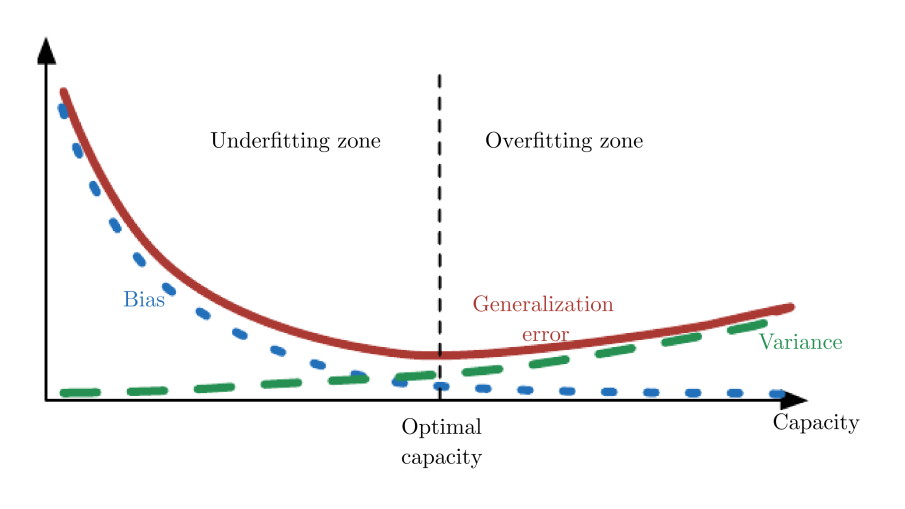
\includegraphics[width=0.8\textwidth]{images/bias_variance_tradeoff.png}
    \caption{}
    \label{fig:}
\end{figure}

As Depicted in the Figure, the Bias and the Variance are inversely proportional. If the Bias is high, the Variance is low and vice versa. The Goal is to find the sweet spot where the Bias and the Variance are both low. This is called the Bias-Variance Tradeoff.

\subsection{Point Estamation and the Consinstency of the Estimator}
A Point Estimator is consistent if it converges in Probability to the true value of the parameter. This means that the Estimator is getting better and better with more data. Formally this is written as $\lim_{m \rightarrow \infty} P(|\hat{\theta}_m - \theta| > \epsilon) = 0$. 

\subsection{Maximum Likelihood Estimation}

The Maximum Likelihood Estimation is a method to estimate the parameter previously discussed. It is defined as $\hat{\theta}_{ML} = \arg \max_{\theta} p_{model}(X|\theta) = \arg \max_{\theta} \prod_{i = 1}^{m} p_{model}(x_{i}|\theta)$. This means that the Maximum Likelihood Estimation maximizes  $ \hat{\theta}_{ML} $ given the data $X$.
With no poof what so ever we will assume, that the Maximum Likelihood Estimation is consistent, when the true distrubution $p_{data} $ is in the model class and $p_{data}$ is a Value of $\theta$ 

\subsection{(Negative) Log Likelihood}

Since it is numerically Problematic to take the Product, due to overflow/underflow we can take the Logarithm of the Likelihood. This is called the Log Likelihood. It is defined as 

\begin{align*}
    \arg\max_{\theta} \log p_{model}(X|\theta) &= \arg\max_{\theta} \log \prod_{i = 1}^{m} p_{model}(x_{i}|\theta) \\
    &= \arg\max_{\theta} \sum_{i = 1}^{m} \log p_{model}(x_{i}|\theta) \\
    \arg\min_{\theta} \left(- \log p_{model}(X|\theta)\right) &= \arg\min_{\theta} \left(- \sum_{i = 1}^{m} \log p_{model}(x_{i}|\theta)\right)
\end{align*}
The last Equation is the Negative Log Likelihood. It is the same as the Log Likelihood, but with a minus sign in front. This is done to make it a minimization Problem, as most Optimization Algorithms are designed to minimize a Function.

\subsection{Negative Log-Likelihood and Cross Entropy}
Negative Log-Likelihood and Cross Entropy are equivalent when m approaches infinity. This is due to the fact that the Negative Log-Likelihood is the average Cross Entropy. This can be shown as follows:
Given that the samples \( x_i \) are drawn from the true data-generating distribution \( p_{data}(x) \), and the negative log-likelihood (NLL) is divided by the number of samples \( m \), the expression for \( m \to \infty \) approximates the cross-entropy between the modeled distribution \( p_{model}(x|\theta) \) and the true data-generating distribution \( p_{data}(x) \):

\begin{align*}
    \frac{1}{m} \sum_{i=1}^{m} - \log p_{model}(x_i|\theta) &\approx \mathbb{E}_{x \sim p_{data}}[-\log p_{model}(x|\theta)] \\
    &= -\int p_{data}(x) \log p_{model}(x|\theta) \, dx \\
    &\approx H(p_{data}, p_{model})
\end{align*}

As \( m \to \infty \), the average NLL converges to the cross-entropy between \( p_{data} \) and \( p_{model} \).

\subsection{Conditional Negative Log-Likelihood}
We can generalize the Negative Log-Likelihood to the Conditional Negative Log-Likelihood. This is done by conditioning the Negative Log-Likelihood on the input. It is defined as $\arg \min_{\theta} \sum_{i = 1}^{m} - \log p_{model}(y_{i}|x_{i}, \theta)$. This is particularly useful, because it can be used in Classification, Segmentation, among many other Tasks, where we want to Intepret the conditional Probability of the output given the input.

\subsection{Cross Entropy for Classification/Segmentation}
In Classification and Segmentation Problems a Neural Network usually learns Probability Function right away lets call it $p_{\theta}(y|x)$ This leads to the following Negative Log Likelihood: $- \log p(Y|X,\theta) =  \sum_{i} - \log p(y_{i}|x_{i}, \theta)$.  
Thus follows the Cross Entropy Loss: $H = \frac{1}{m} \sum_{i} - \log p_{\theta}(y_{i}|x_{i})$
\subsection{Segmentation and Pixel Wise Classification}
In Segmentation and Pixel Wise Classification the Cross Entropy Loss is calculated for every Pixel. This is done by calculating the Cross Entropy Loss for every Pixel and then averaging over all Pixels. This is done to get a single Value for the Loss.
\begin{figure}[h]
    \centering
    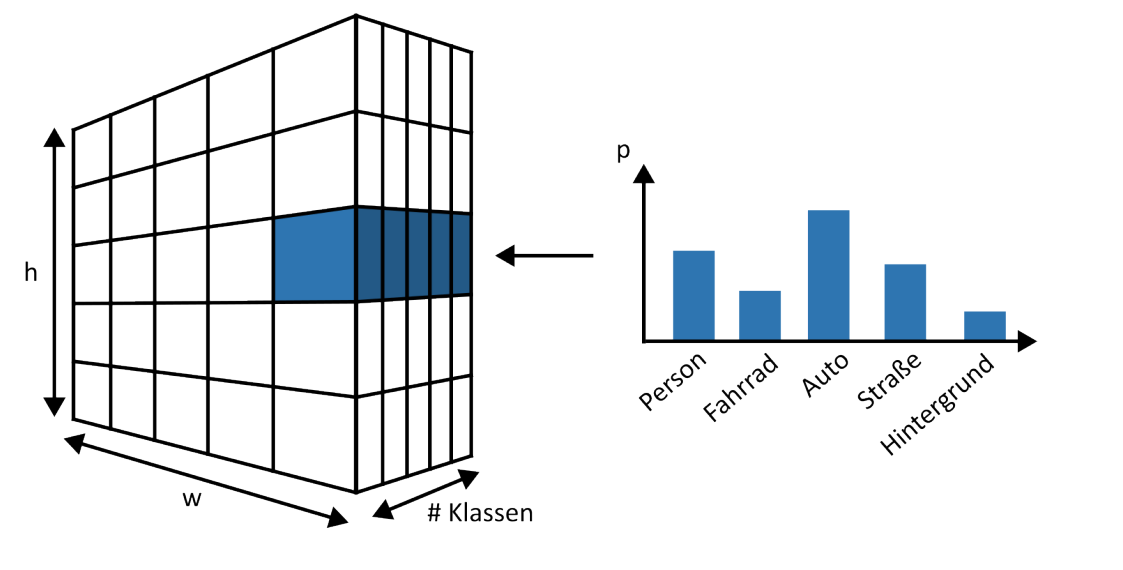
\includegraphics[width=0.8\textwidth]{images/pixel_wise.png}
    \caption{}
    \label{fig:}
\end{figure}
The Figure is a visualization of the Cross Entropy Loss for a Pixel Wise Classification Task. Every Layer here represents a Class. So here the average for all Classes is calculated and then compared to get a Classification Result. 

\subsection{Mean Squared Error for Regression}
If we consider the Normal Distribution as the Model Distribution, the mean of that is learned by the Neural Networks, considering most Regression Problems. This leads to the Likelihood being defined as $p(Y|X,\theta, \sigma) = \prod_{i} \mathcal{N}(y_{i},\mu_{\theta}(x_{i}),\sigma)$
Thus follows the Negative Log Likelihood: $- \log p(Y|X,\theta, \sigma) =  \sum_{i} \frac{1}{2} 2(\pi \sigma^{2}) + \frac{1}{2} \frac{(y_{i} - \mu_{i}(x_{i}))^{2}}{\sigma^{2}}$. If we assume that the Variance is constant, we can drop the first term, also the Denominator can be dropped, as it is constant aswell. This leads to the Mean Squared Error: $MSE = \frac{1}{m} \sum_{i} (y_{i} - \mu_{i}(x_{i}))^{2}$
The minimum of the Mean Squared Error is if $\mu(x_{i}$ is the mean of the samples.)


\subsection{Mean Absolute Error}
For the MAE or $L{1}$ a Laplace Distribution is assumed. This leads to the Likelihood being defined as $p(Y|X,\theta, \sigma) = \prod_{i} \mathcal{L}(y_{i},\mu_{\theta}(x_{i}),\sigma)$ With the NLL being defined as $- \log p(Y|X,\theta, \sigma) =  \sum_{i} log(2 \sigma) + \frac{|y_{i} - \mu_{i}(x_{i})|}{\sigma}$. This leads to the Mean Absolute Error: $MAE = \frac{1}{m} \sum_{i} |y_{i} - \mu_{i}(x_{i})|$ The Major difference is the missing squared making it more robust to outliers. But also the minimum is not the mean of the samples, but the median. 

\subsection{Maximum A Posteriori Estimation}
An alternative to the Maximum Likelihood Estimation is the Maximum A Posteriori Estimation. It is defined as $\hat{Theta}_{MAP} = \arg \max _{\theta} p(\theta|X)$
Assuming $\theta$ is a random variable, we can use Bayes Rule to rewrite this as $\hat{\theta}_{MAP} = \arg \max _{\theta} p(X|\theta) p(\theta)$ To further simplify the operations, we can take the log as per usual. This leads to $\hat{\theta}_{MAP} = \arg \max _{\theta} \log p(X|\theta) + \log p(\theta)$ Here we can incoperate a sum again thus follows $\hat{\theta}_{MAP} = \arg \max _{\theta} \sum_{i} \log p(x_{i}|\theta) + \log p(\theta)$
The is as the Name already hints, the Maximum Likelihood Estimation with a Prior. This is useful if we have some prior knowledge about the parameter. With backround knowledge we can push $\theta$ to a realistic value. Say we have knowledge X we can have  $P(Y|X,\theta)$ here the same with x follows $\hat{\theta}_{MAP} = \arg \max _{\theta} \sum_{i} \log p(x_{i}|x_{i}\theta) + \log p(\theta)$
This is a key Concept later on for Regularization of Weights for Neural Networks.

\section{Error functions}
The NLL  $\hat{\theta}_{ML} =  \arg\min_{\theta} (- \sum_{i = 1}^{m} \log p(x_{i}|\theta)) = \arg \min_{\theta} f(\theta)$ the Maximum Likelihood Estimator will now be viewed as the minimum of a Function. One might notice that this does not look too different from minimizing or maximizing a function during Training in Machine-Learning. This would in that Context be reffered to as  Objective Function, cost function, error function or loss function. The Variable $\theta$ that is to be Optimized would then be equivalent to the Parameters of the Model. Thus the Maximum Likelihood Point Estimation is equivalent to a Machine Learning Algorithm. 
The obvious question now is, how do we minimize this function?



\subsection{Local and Global Minima}
\begin{figure}[h]
    \centering
    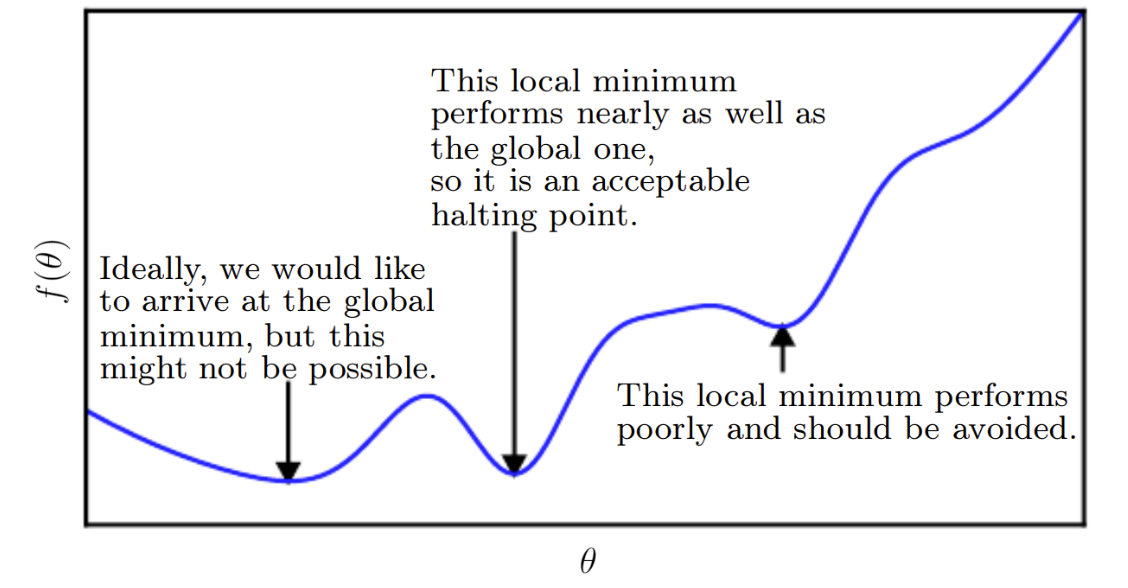
\includegraphics[width=0.8\textwidth]{images/local_global.png}
    \caption{}
    \label{fig:Local vs Global Minima}
\end{figure}
As explained before the Local Minima is the one found by Gradient Descent. This might not be too bad if it is approximitely the same as the Global Minima. But if it is not, the Algorithm will get stuck in the Local Minima. A good rule of thumb is to compare the Local Minima to low values of the cost function, if they are not far off, the Local Minima is good enough.

\newpage
\subsection{Convex Functions}
Convex function if $\forall x,y \in D  \text{and} t \in [0,1] \rightarrow f(tx + (1-t)y) \leq tf(x) + (1-t)f(y)$ hold. This basically just means that every point is below the average of the two points. Convex Functions have the nice property that they have only one minimum. However this is rather rare in the context of Machine Learning.


\begin{figure}[h]
    \centering
    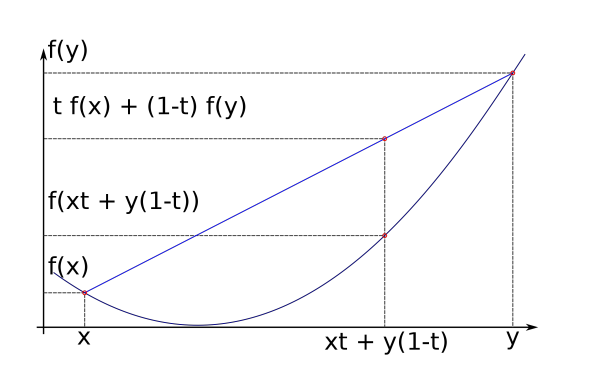
\includegraphics[width=0.8\textwidth]{images/convex.png}
    \caption{}
    \label{fig: Illustration of Convexity}
\end{figure}

\subsection{Different approaches to find Minima}

\subsubsection{Least Squares}
Least Squares is a method to find $\hat{\theta}$ for a linear Model this is done by taking $\arg \min_{\theta} ||A \theta - y ||^{2} = (A^{*}A)^{-1} A^{*}y$ This only works for least squares though and Machine Learning Models are usually not linear.

\subsubsection{Grid Search}
Grid Search is a method to find the minimum of a function. It is done by evaluating the function at every point on a grid. This is rather slow, as the number of points grows exponentially with the number of dimensions.

\subsubsection{Evoluationary Algorithms}
Evolutionary Algorithms are a class of algorithms that are inspired by the process of natural selection. They work by creating a population of solutions and then using genetic operators such as mutation and crossover to evolve the population over time. This is rather slow aswell, as it is a brute force method. It works fine for 10-1000 Parameters but becomes inneficient for more. It can be usefull for HyperParameters though. 

\subsubsection{Gradient Based Optimization}
If the Model and the Error Function are differentiable, Gradient Based Optimization can be used. This is done by calculating the Gradient of the Error Function and then following the Gradient to the minimum.

\section{Gradient Descent}
\subsection{Error Surface}

\begin{figure}[h]
    \centering
    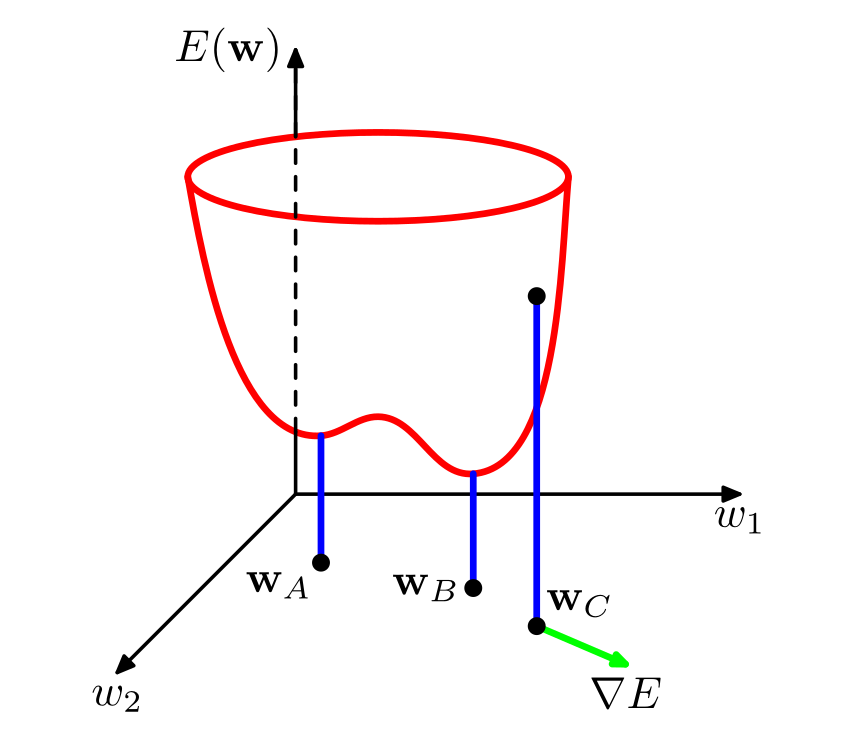
\includegraphics[width=0.8\textwidth]{images/error_surface.png}
    \caption{}
    \label{fig:Error Surface}
\end{figure}

This is a Geometric Representation of the Errror Function. $w_{A} , w_{B}$ is a local and a Global minimum. Here Gradient Descent comes in handy. If we start at a random point, here $w_{C}$ we can follow the Gradient to the minimum. So basically we just find the derivative of the function, follow the Gradient to the opposite direction and repeat this until we reach the minimum. The opposite direction is taken, as the Gradient points to the steepest ascent, and for minimization we want to go in the opposite direction.

\subsection{Formal Definition of Gradient Descent}
We are looking for $\theta$ that minimizes the Error Function $f(\theta)$ Since we can not do this analytically we will use a numerical method.  For that we choose a starting value $\theta_{0}$ and then update it iteratively. The update rule is defined as $\theta_{i+1} = \theta_{i} + \Delta \theta_{i}$ 
The usual way to do this is to introduce a learning rate $\epsilon$ and then update the parameter as follows $\theta_{i+1} = \theta_{i} - \epsilon \nabla f(\theta_{i})$

\subsection{Gradient - Taking the Derivative in Multiple Dimensions}
The Error Function of a Neural Net is usually dependent on multiple Parameters. This is why it becomes necessary to talk about partial derivatives, thus the concept of Gradients is introduced. Let $f(\theta)$ be a skalar Function. Meaning it mapps from $\mathbb{R}^{n} \rightarrow \mathbb{R}$. The Gradient of $f$ is defined as $\nabla f(\theta)_{i} = \frac{\partial f(\theta)}{\partial \theta_{i}} f(\theta)$ This is just the partial derivative of $f$ with respect to $\theta_{i}$. If u write this in vector form it becomes $\nabla f(\theta) = \begin{pmatrix} \frac{\partial f(\theta)}{\partial \theta_{1}} \\ \frac{\partial f(\theta)}{\partial \theta_{2}} \\ \vdots \\ \frac{\partial f(\theta)}{\partial \theta_{n}} \end{pmatrix}$ So every entry of the Gradient is the partial derivative of $f$ with respect to the corresponding parameter in our cases usually the weight.
A stationary point is given if every entry of the Gradient is 0.

\subsection{Direcional Derivative}
The Directional Derivative describes the rate in which a function changes in a certain direction. It is defined as $\nabla_{u} f(\theta) = \lim_{\alpha \rightarrow 0} \frac{f(\theta + \alpha u) - f(\theta)}{h}$ This is just the derivative of $f$ in the direction of $u$. This can be rewritten as $\nabla_{u} f(\theta) = \nabla f(\theta) u^{T}$ This is just the dot product of the Gradient and the direction.
To minimize f, we must find the direction u, where f decreases the fastest, this means $min_{u,u^{T}u =1} \ u^{T} \nabla f(\theta) = min_{u,u^{T}u =1} ||u||_{2} \cdot ||\nabla f(\theta)||_{2} \cdot \cos(\phi) $.
where $\phi$ is the angle between the Gradient and the direction. Since u is a unit vector, the minimum can be simplified to $min_{u} \cos(\phi)$, since the Gradient is independent of u. This is due to the fact that $\cos$ oxcilates between -1 and 1. Thus the minimun is -1 and $\cos(\pi) = -1$ 

\subsection{Learning Rate $\epsilon$}
For now we will have  just take $\epsilon$ as a small constant. The danger when $\epsilon$ is too large is that may not converge to the minimum. If $\epsilon$ is too small, the convergence will be slow. This is why it is important to choose $\epsilon$ wisely.

\subsection{Jacobi Matrix}
If we now have vectors as inputs and outputs it is handy to define a Matrix called Jacobi-Matrix. This matrix conatins the partial derivative of f at the position x. It is defined as \[ (J_{f}(\theta))_{i,j} = \frac{\partial}{\partial \theta_{j}} f(\theta)_{i} \]
This can be written in the following Matrix Form \[ J_{f}(\theta) = \begin{pmatrix} \frac{\partial f_{1}(\theta)}{\partial \theta_{1}} & \frac{\partial f_{1}(\theta)}{\partial \theta_{2}} & \cdots & \frac{\partial f_{1}(\theta)}{\partial \theta_{n}} \\ \frac{\partial f_{2}(\theta)}{\partial \theta_{1}} & \frac{\partial f_{2}(\theta)}{\partial \theta_{2}} & \cdots & \frac{\partial f_{2}(\theta)}{\partial \theta_{n}} \\ \vdots & \vdots & \ddots & \vdots \\ \frac{\partial f_{m}(\theta)}{\partial \theta_{1}} & \frac{\partial f_{m}(\theta)}{\partial \theta_{2}} & \cdots & \frac{\partial f_{m}(\theta)}{\partial \theta_{n}} \end{pmatrix} \]

\subsection{The Derivative of second order}
The derivative of second order is important for us as well since it can imply the improvement that is expected of one iteration of the Gradient Descent. 

\subsection{Hessian Matrix}
The Hessian Matrix is the Matrix of second order partial derivatives of a function. It is defined as \[ H_{f}(\theta)_{i,j} = \frac{\partial^{2}}{\partial \theta_{i} \partial \theta_{j}} f(\theta) \] The directional Derivative of second order to a Directionvector u 
is given by $u^{T} H_{f}(\theta) u$. If u is an Eigenvektor of H, then the derivative of second order is equivalent to the corresponding Eigenvalue. For other directions, the derivative of second order is the weighted average of the Eigenvalues.
Where Directions which correspond better with the Eigenvalues are more important. This also implies that the second directional derivative is beween the smallest and the largest Eigenvalue of H, because it is a weighted sum, it must be contrained by the smallest and the largest Eigenvalue.

This is also equivalent to the Jacobi Matrix of the Gradient. 

\subsection{Approximate Second-Order Methods}
Let's have a look at the Newton Method. The Newton Method is used to find the minimum of a function. It is defined as $\theta_{i+1} = \theta_{i} - H_{f}(\theta_{i})^{-1} \nabla f(\theta_{i})$ This is just the Gradient Descent with the Hessian Matrix. 
I mean it makes sense though, since we basically exchanged our shitty $\epsilon$ to a more dynamic way of choosing the learning rate. 
It brings some disatvantages though, as the Hessian Matrix calculation as well as the inversion can be rather expensive for large disatvantages. 

\section{Stochastic Gradient Descent}
If the calculation of the Gradient is done for the entire Dataset, it might be slow, due to the immense size. Also the data during an iteration is saved in RAM or Graphicsmemory, this can be become impossible to handle for large Datasets. This is why we introduce Stochastic Gradient Descent. Which takes Batches of the Data and calculates the Gradient for these Batches. 
Lets assume that the Trainingsample is i.i.d. then the log likelihood can be written as $L_{\theta}(X) = \frac{1}{n} \sum_{i=1}^{n} L(f_{\theta}(x_{i}),y_{i})$ which implicates that the Gradient can be written as $\nabla_{\theta} L_{\theta}(X) = \frac{1}{n} \sum_{i=1}^{n} \nabla_{\theta} L(f_{\theta}(x_{i}),y_{i})$ This is just the average of the Gradients of the Batches. 

\subsection{Mini-Batch Gradient as an unbiased Estimator}
The Approximation of the Gradient with the help of Mini-Batches can be seen as an unbiased Estimator of the Gradient. In math language we can write 
\begin{align*}
    \mathbb{E} \left[ \nabla_{\theta} L_{\theta} (\hat{X}) \right] 
    &= \mathbb{E} \left[ \frac{1}{k} \sum_{x \in \hat{X}} \nabla_{\theta} L_{\theta} (x) \right] \\
    &= \frac{1}{|\mathcal{X}_k|} \sum_{\hat{X} \in \mathcal{X}_k} \frac{1}{k} \sum_{x \in \hat{X}} \nabla_{\theta} L_{\theta} (x) \\
    &= \frac{1}{k} \sum_{x \in X} \frac{\binom{n-1}{k-1}}{\binom{n}{k}} \nabla_{\theta} L_{\theta} (x) \\
    &= \frac{1}{k} \sum_{x \in X} \frac{k}{n} \nabla_{\theta} L_{\theta} (x) \\
    &= \frac{1}{n} \sum_{x \in X} \nabla_{\theta} L_{\theta} (x) \\
    &= \nabla_{\theta} L_{\theta} (X)
    \end{align*}
    The given equations demonstrate that the expected gradient of the loss function, when computed over a randomly sampled subset of the data, equals the gradient of the loss function over the entire dataset. This result shows that using mini-batches in stochastic gradient descent  provides an unbiased estimate of the full gradient. As a result, SGD can efficiently and effectively optimize the model parameters by using only small subsets of data at each iteration, making it scalable and practical for large datasets.
    (rewritten by chatgpt so it becomes more coherent lol)


\subsection{Batch Size}
The Batch size is as per usual a trade off, either we choose large Batches. This would lead to a more accurate Gradient, but needs to more computation power. If we choose small Batches, the Gradient is less accurate, but the computation is faster. This makes it necessary to choose a smaller learning rate so the training remains stable.
For the Varianz of the Gradient $Var(\frac{1}{|I|} \sum_{i\in I} g_{i}) = \frac{1}{|I|^{2}}\sum_{i\in I}Var(g_{i})= \frac{\sigma^{2}}{|I|}$
I is a set of indices of the Patch and the Gradients are $g_{i}$ This makes sense as it exactly depicts the relation we established before the equation.
The choice of the Batch size, since it is a Tradeoff depends on several Factors
\begin{enumerate}
    \item If the Batches are processed in parallel, the Batch size should be chosen to fit the memory of the GPU.
    \item Multiprozessor Systems can't be used to their full potential if the Batch size is too small. Since the Batches have fixed cost for the computation at a certain size. 
    \item Hardware is optimized for certain Batch sizes. For GPUs this is usually $2^{n}$.
    \item Small Batches have a Regularization effect, as the Gradient is more noisy.
\end{enumerate}

\subsection{Algorithm for Stochastic Gradient Descent}
\begin{algorithm}[h]
    \caption{Stochastic gradient descent (SGD) update at training iteration $k$}
    \begin{algorithmic}
    \Require Learning rate $\epsilon_k$
    \Require Initial parameter $\theta$
    \While{stopping criterion not met}
        \State Sample a minibatch of $m$ examples from the training set $\{ x^{(1)}, \ldots, x^{(m)} \}$ with corresponding targets $y^{(i)}$
        \State Compute gradient estimate: $\hat{g} \leftarrow \frac{1}{m} \nabla_\theta \sum_{i} L(f(x^{(i)}; \theta), y^{(i)})$
        \State Apply update: $\theta \leftarrow \theta - \epsilon \hat{g}$
    \EndWhile
    \end{algorithmic}
    \end{algorithm}
    Lets go through the Algorithm step by step. First we give a learning rate and an initial parameter. Then we sample a minibatch of m examples from the training set. We compute the gradient estimate by taking the average of the gradients of the loss function over the minibatch. We then apply the update rule to the parameter by subtracting the learning rate times the gradient estimate. We repeat this process until a stopping criterion is met, which could be a maximum number of iterations, a convergence criterion, or another condition.

    \subsection{Learning Rate $\epsilon$}
    The first Parameter was the Learning Rate $\epsilon$. The Learning Rate needs to go to Infinity, so $\sum_{k=1}^{\infty} \epsilon_{k} = \infty$ and $\sum_{k=1}^{\infty} \epsilon = \infty$ Usually the learning rate is being reduced over time. This is done by a learning rate schedule. For example a linear decay, where the learning rate is reduced by a contant factor until it reaches a certain iteration, where is remains constant. 

    \subsection{Momentum}
    \subsection{Algorithm for Stochastic Gradient Descent with Momentum}
    Momentum is a method to accelerate the convergence of Gradient Descent. Momentum aggregates the Gradients of previous Iterations. $$v \leftarrow \alpha v + \epsilon \nabla_{\theta}(\frac{1}{m} \sum_{i=1}^{m} L(f(\theta^{(i)};\theta),y^{(i)})) $$ This is just the Gradient Descent with the addition of the Momentum. The Momentum is a Hyperparameter and is usually set to 0.9, 0.99, or 0.5. The Momentum is then used to update the parameter as follows $\theta \leftarrow \theta + v$ This is just the Gradient Descent with the addition of the Momentum. The Momentum is a Hyperparameter and is usually set to 0.9, 0.99, or 0.5. The Momentum is then used to update the parameter as follows $\theta \leftarrow \theta - v$
    \begin{algorithm}
\caption{Stochastic gradient descent (SGD) with momentum}
\begin{algorithmic}
\Require Learning rate $\epsilon$, momentum parameter $\alpha$
\Require Initial parameter $\theta$, initial velocity $v$
\While{stopping criterion not met}
    \State Sample a minibatch of $m$ examples from the training set $\{ x^{(1)}, \ldots, x^{(m)} \}$ with corresponding targets $y^{(i)}$
    \State Compute gradient estimate: $g \leftarrow \frac{1}{m} \nabla_\theta \sum_i L(f(x^{(i)}; \theta), y^{(i)})$
    \State Compute velocity update: $v \leftarrow \alpha v - \epsilon g$
    \State Apply update: $\theta \leftarrow \theta + v$
\EndWhile
\end{algorithmic}
\end{algorithm}
\section{Adaptive Learning Rates}
This basically just means that we can adapt the learning rate to the Parameters. There are several methods to do this. 
\begin{enumerate}
    \item AdaGrad scales a learning rate by the inverse of the square root of the sum of all historical squared gradients. This means that the learning rate is reduced for parameters that have received large gradients in the past.
    \item RMSProp is similar to AdaGrad, but uses a moving average of squared gradients instead of the sum of squared gradients. This allows the learning rate to adapt more quickly to changes in the gradients.
    \item Adam combines the ideas of momentum and RMSProp. It uses a moving average of gradients and a moving average of squared gradients to adapt the learning rate for each parameter. 
\end{enumerate}
\subsection{AdaGrad Algorithm}
\begin{algorithm}
    \caption{The AdaGrad algorithm}
    \begin{algorithmic}
    \Require Global learning rate $\epsilon$
    \Require Initial parameter $\theta$
    \Require Small constant $\delta$, perhaps $10^{-7}$, for numerical stability
    \State Initialize gradient accumulation variable $r = 0$
    \While{stopping criterion not met}
        \State Sample a minibatch of $m$ examples from the training set $\{ x^{(1)}, \ldots, x^{(m)} \}$ with corresponding targets $y^{(i)}$
        \State Compute gradient: $g \leftarrow \frac{1}{m} \nabla_\theta \sum_i L(f(x^{(i)}; \theta), y^{(i)})$
        \State Accumulate squared gradient: $r \leftarrow r + g \odot g$
        \State Compute update: $\Delta \theta \leftarrow -\frac{\epsilon}{\delta + \sqrt{r}} \odot g$ \hspace{0.2cm} (Division and square root applied element-wise)
        \State Apply update: $\theta \leftarrow \theta + \Delta \theta$
    \EndWhile
    \end{algorithmic}
    \end{algorithm}
    So the steps added here are the Accumulation of the squared Gradient, and the update. As mentioned in the short description before, since the Multiplikation and the Division are applied element wise, the update is done for every parameter and so every parameter that was previosuly large will have a reduced learning rate. The other algorithms for other adaptive learning rates are similar to this one, but with the steps I descibed before.
    \section{Feed-Forward Networks}

    \subsection{Single-Neuron}

    The output of  single Neuron with D input values $x_{i}$, weights $w_{i}$ and Bias b can be calculated as follows: $$a = \sigma(\sum_{i=1}^{D} w_{i}x_{i} + b)$$ where $\sigma$ is the activation function. The activation function is usually a non-linear function, such as the sigmoid function, the tanh function, or the ReLU function. The output of the neuron is then passed through the activation function to produce a non linear output. This is done, so that the Model can learn non-linear relationships between the input and the output, otherwise the Model would just be a linear regression.

    \subsection{One Layer and multiple Neurons}
    Often a layer is defined by Multiple Neruons, those are fed with the same input and combined in one layer. The output of such a layer can be calculated by $$a = \sigma(\sum_{i=1}^{D}w_{ji} \cdot x_{i} + b_{j})$$ The Compact form of this would be $a = \sigma(Wx + b)$ where $W$ is the Matrix of the weights and $b$ is the Bias.


    \subsection{Multiple Layers}

    Well, now that we have the defenition of one Layer down, why not do Multiple and thus create a neural Net. The output of a Neural Net with L layers can be calculated as follows: \begin{align*}
        a^{(1)} &= \sigma(W^{(1)}x + b^{(1)}) \\
        a^{(2)} &= \sigma(W^{(2)}a^{(1)} + b^{(2)}) \\
        &\vdots \\
        a^{(L)} &= f^{out} (W^{(L)}a^{(L-1)} + b^{(L)})
    \end{align*}
    Now we can consider writing this as a parameterized function
  
    \[
\text{nn}_{\theta}(x) = f_{\text{out}} \left( W^{(N)} \cdot f^{(N-1)} \left( \ldots W^{(2)} \cdot f^{(1)} \left( W^{(1)} \cdot x + b^{(1)} \right) + b^{(2)} \ldots \right) + b^{(N)} \right)
\]

With the parameters:

\[
\theta = \left( (W^{(1)}, b^{(1)}), (W^{(2)}, b^{(2)}), \ldots, (W^{(N)}, b^{(N)}) \right)
\]
The f I use is just a placeholder for the activation function.

How many layers exist is something we will define with the amount of layers being the amount of weight matrices used for Multiplication. 

\subsection{Fun Facts for Linear Activation}
Lets say we decide to use a linear function, lets show by its properties that it is not a good choice. 

\[
\text{nn}_{\theta}(x) = f_{\text{out}}\left(W^{(N)} \cdot f^{(N-1)}\left(\cdots f^{(2)}\left(W^{(2)} \cdot f^{(1)}\left(W^{(1)} \cdot x\right)\right)\right)\right)
\]

This can be simplified by grouping the weight matrices and activation functions:

\[
\text{nn}_{\theta}(x) = f_{\text{out}}\left(W^{(N)} \cdot f^{(N-1)}\left(\cdots f^{(2)}\left(W^{(2)} \cdot W^{(1)} \cdot f^{(1)}(x)\right)\right)\right)
\]

Combining weights into a single matrix \(W'\):

\[
\text{nn}_{\theta}(x) = f_{\text{out}}\left(W^{(N)} \cdots W^{(2)} \cdot W^{(1)} \cdot f^{(N-1)} \circ f^{(2)} \circ f^{(1)}(x)\right)
\]

Finally, we get:

\[
\text{nn}_{\theta}(x) = f_{\text{out}}\left(W' g(x)\right)
\]

\subsection{Activation Functions}
The Activation Function is a non-linear function that is applied to the output of a neuron. As shown before we do need those non-linear Activation Functions to learn non-linear relationships. We can differentiate beween two Sorts of here, one being for Hidden Layers (So the Layers between the Input and the Output) 
and the other for the Output Layer. Some of the Hidden Layer Activation Functions are:
\begin{itemize}
    \item Sigmoid: $\sigma(x) = \frac{1}{1 + e^{-x}}$
    \item Tanh: $\tanh(x) = \frac{e^{x} - e^{-x}}{e^{x} + e^{-x}}$
    \item ReLU: $ReLU(x) = \max(0,x)$
    \item Hard Tanh: $HardTanh(x) = \max(-1, \min(1,x))$
    \item Softplus: $Softplus(x) = \log(1 + e^{x})$
    \item 
\end{itemize}
Some of the Output Layer Activation Functions are:
\begin{itemize}
    \item Linear: $f(x) = x$
    \item Sigmoid: $\sigma(x) = \frac{1}{1 + e^{-x}}$
    \item Softmax: $Softmax(x) = \frac{e^{x_{i}}}{\sum_{j} e^{x_{j}}}$
\end{itemize}
For the output Functions it is maybe important to note that you can use the Sigmoid Function for Binary Classification and the Softmax Function for Multiclass Classification. 

\subsection{Symmetries in Parameter Space}
There are many ways to achieve the same mapping of input to output values, even though the weight matrices and biases are different. One way is to permute the neurons in a layer, this leads to $M!$ equivalent solutions. Some activation functions are also point reflections, meaning that $f(x) = f(-x)$, this leads to $2^{M}$ equivalent solutions. 
An Example for this would be $tanh(-x) = -tanh(x)$ If we combine those symmetries, we get $2^{M} \cdot M!$ equivalent solutions. This also there are as many equivalent local Minima. Which is ok though, as large networks local Minimas are usually quite good. 

\subsection{Universal Approximation Theorem}
This Theorem  states that if we have 2 layers, with enough hidden units, 
we can approximate any Continuous Function.

\section{Backpropagation}
\subsection{Why do we need Backpropagation?}
 As discussed in Chapter 5 we use gradient descent to minimize the error function. The error function is a function of the parameters of the model, and we need to compute the gradient of the error function with respect to the parameters in order to update them. 
 Perhaps a rather simple approach would be to to calculate the Difference quotient being defined by $$\frac{\partial L}{\partial W_{ji}} = \frac{L(W_{ji} + \epsilon) - L(W_{ji} - \epsilon)}{2 \epsilon} + \underbrace{O(\epsilon^{2})}_{residual \ corrections}$$ This is a rather simple approach, but it is not very efficient, since you need to evaluate the Loss-Function twice for every Parameter. As this is why we use the Backpropagation Algorithm.

 \subsection{Lets look at the Chain Rule}
 For Backpropagation we first need to understand the chain rule. The chain rule in 1D is defined as $(g \circ f)' (x) = g' (f(x)) \cdot f'(x)$. This is also written as $\frac{x}{\partial x} g(f(x)) = \frac{\partial g}{\partial f} \frac{\partial f}{\partial x}$.
 If our function depends on multiple variables, for example $x$ and $y$ then we can look at the partial derivatives. Meaning the partial derivative of $f(x,y) $ with respect to $x$ can be written as $\frac{\partial f}{\partial x}$. And with respect to $y$ as $\frac{\partial f}{\partial y}$. 

 \newpage
 \subsection{Direcional Derivative with the Chain Rule}
 \begin{figure}[h]
    \centering
    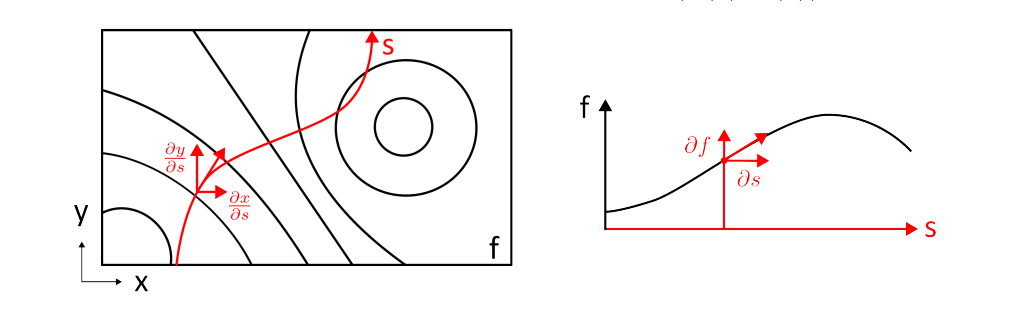
\includegraphics[width=0.8\textwidth]{images/richtungsableitung.png}
    \caption{}
    \label{fig:Richtungsableitung}
\end{figure}
Ok lets say our goal is to calculate the partial derivative of f to s, on the left graph.  Well to analyze we take the chain rule, meaning we can express $f$ as $f(x(s),y(s))$ and can then write the partial derivative of $f$ with respect to $s$ so $\frac{\partial f}{\partial s} = \frac{\partial f}{x} \frac{\partial x}{\partial s} + \frac{\partial f}{\partial y} \frac{\partial y}{\partial s}$. This is just the chain rule applied to the partial derivatives.
So if more Dimensions follow, we can use the same pattern. 
\begin{center}
    

\begin{tikzpicture}
    % Nodes
    \node (s) at (0,0) {$s$};
    \node (x) at (3,2) {$x(s)$};
    \node (y) at (3,0) {$y(s)$};
    \node (z) at (3,-2) {$z(s)$};
    \node (f) at (6,0) {$f(x,y,z)$};
    
    % Arrows
    \draw[->] (s) -- (x) node[midway, above, sloped] {$\frac{\partial x}{\partial s}$};
    \draw[->] (s) -- (y) node[midway, above] {$\frac{\partial y}{\partial s}$};
    \draw[->] (s) -- (z) node[midway, above, sloped] {$\frac{\partial z}{\partial s}$};
    \draw[->] (x) -- (f) node[midway, above, sloped] {$\frac{\partial f}{\partial x}$};
    \draw[->] (z) -- (f) node[midway, above, sloped] {$\frac{\partial f}{\partial z}$};
    
    % Equation
    \node at (0, -4) {
    \begin{minipage}{\textwidth}
    \begin{equation*}
        \frac{\partial f}{\partial s} = \frac{\partial f}{\partial x} \frac{\partial x}{\partial s} + \frac{\partial f}{\partial y} \frac{\partial y}{\partial s} + \frac{\partial f}{\partial z} \frac{\partial z}{\partial s}
    \end{equation*}
    \end{minipage}
    };
    
\end{tikzpicture}
\end{center}
This concept can easily be expanded to more functions, lets say we also have $g$ we then need to calculate $g$ in respect to $s$, to do this we can say $$\frac{g}{\partial s} = \frac{\partial g}{\partial f} \frac{\partial f}{\partial s}$$  Since I had trouble understanding it, lets make a quick example for $g$ and $f$. 
If g and f are dependent on one variable s. 
\[
f(s) = s^2
\]
\[
g(f) = f + 1
\]

We want to find \(\frac{\partial g}{\partial s}\).


1. Compute \(\frac{\partial f}{\partial s}\):
\[
\frac{\partial f}{\partial s} = \frac{\partial (s^2)}{\partial s} = 2s
\]

2. Compute \(\frac{\partial g}{\partial f}\):
\[
\frac{\partial g}{\partial f} = \frac{\partial (f + 1)}{\partial f} = 1
\]

3. Apply the chain rule:
\[
\frac{\partial g}{\partial s} = \frac{\partial g}{\partial f} \cdot \frac{\partial f}{\partial s} = 1 \cdot 2s = 2s
\]

Thus, the derivative of \(g\) with respect to \(s\) is:
\[
\frac{\partial g}{\partial s} = 2s
\]
With more variables and more functions this becomes increasingly annoying to write down, which is why it looks so complicated in the Slides. But with Neural Nets we typically have many layers, thus making these "graphs" unsuitable for the task.
Now this where Backpropagation finally comes in handy.
\subsection{Backpropagation Algorithm Intuitively}
Well lets talk about Backpropagation in a more intuitiv manner before discussing the calculus involved. We first run the forward pass so we pass in Training examples and then calculate the output of the Neural Net. If we think of classifiying a number for example, this will most likely not be the correct output. So we calculate the error of that output thus giving us the loss, so how far off our predictions are from the actual values.
Ok now we can apply the backward pass. We basically go back through the layers and check where mistakes were made. Thus we calculate how much each weight in the network contributed to the error. So now we can adjust the weights to minimize the loss in the Neural Net. We can do this over and over again for each Training example, until the loss is minimized. Chapter 3 of the 3B1B Video Series on Neural Networks might be worth to check out. 


\subsection{Backpropagation Algorithm Formally}

\begin{figure}
    \centering
    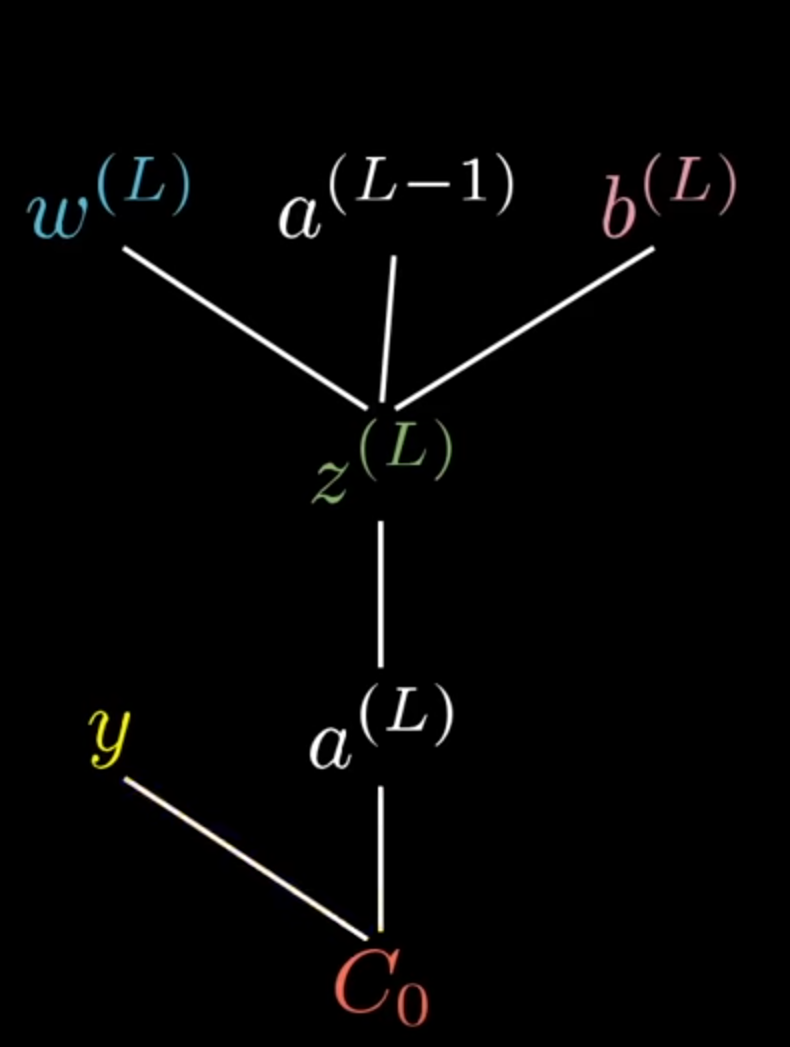
\includegraphics[width=0.8\textwidth]{images/3b1b_backpropagation.png}
    \caption{3B1B Backpropagation}
    \label{fig:Backpropagation}
\end{figure}

Ok lets first look at simple example and then expaldn it, lets say we only have 1 Neuron per layer now lets introduce some notations, as shown in the image. Lets focus on the connection of the last 2 Neurons first. $a^{L}$ being the activation of the last neuron, and $a^{(L-1)}$ being the activation of the previous neuron. So how do we determine the last activation well as we discussed it is determined by a weight $w^{(L)}$ the previous action $a^{(L-1)}$ and a bias $a=b^{(L)}$ and then an activation function. We also dicussed that we define a name for that here being $z^{(L)} = w^{(L)} \cdot a^{(L-1)} + b^{(L)}$ and $a^{(L)} = \sigma(z^{(L)})$. 
Now that we computed a as shown in the image we can compute the cost with a target value $y$ and a cost function $C$ This can be expanded to substituting the $a^{L-1}$ function as well of course. But lets focus on the last layer for now. The first thing that might be interesting here is how changes in the weight effect our cost function. In mathematical Terms we are 
interested in the derivative of the cost function with respect to the weight. $ \frac{\partial C_{0}}{\partial W^{(L)}}$ But how do we get there again with intuition the chain rule makes perfect sense here because what is important for that ratio to know. Well first $w^{(L)}$ effects $z^{(L)}$ which in turn effects $a^{(L)}$ which in turn effects the cost function. 
So lets write this down mathematically using the chain rule! 

\[
\frac{\partial C_{0}}{\partial W^{(L)}} = \underbrace{\frac{\partial z^{(L)}}{\partial w^{(L)}}}_{\shortstack{effect of \( w \) \\ with respect to \( z \)}} \underbrace{\frac{\partial a^{(L)}}{\partial z^{(L)}}}_{\shortstack{now that \( z \) changed \\ let's calculate the effect \\ that has on \( a \)}} \underbrace{\frac{\partial C_{0}}{\partial a^{(L)}}}_{\shortstack{effect of \( a \) \\ on the cost \( C_{0} \)}}
\]
Lets break down the terms now. So first the effect of a on the term C is just $2(a^{(L)} - y)$ The derivative of the activation function is just the derivative of the activation function. And the derivative of $z$ with respect to $w$ is just $a^{(L-1)}$. Because this relation just depends on ow strong the previous neuron was activated. Now this is just for a single training example if we wanted to compute this for 
all the Training examples we would compute an average meaning $$\frac{\partial C}{\partial W^{(L)}} = \frac{1}{n} \sum_{k = 0}^{n-1} \frac{\partial C_{k}}{\partial W^{(L)}}$$ Now we have succesfully computed one component of the gradient vector $C$ We would now need to do the same for the bias and the previous layers. For the bias the computation 
is almost the same, because we can just swap out every w for a b. But if we consider the derivative of $\frac{\partial z^{(L)}}{\partial b^{(L)}}$ we see that this is just 1. Because obviosuly a change in the Bias would result in a change of the activation exactly equivalent to the change in the Bias. Ok now lets look at how we go backward. The sensitivity of the cost function with respect to the activation of the last layer. In the formula it would look like this: \[ \frac{\partial C_{0}}{\partial a^{(L-1)}} = \frac{\partial z^{(L)}}{\partial a^{(L-1)}} \dots \] which in turn would just be the weight. Now since we kept track 
of this we can trace back how sensitive the cost function is to the activation of the previous layer. This is the basic idea of Backpropagation. Now this can be expanded to multiple neurons, however the Idea stays the same. One thing that changes is the cost function with respect to the activation of the previous layer. Lets introduce a new indeci to keep track which neuron talking about lets call it activation of the kth neuron in the L-1 layer with $a_k^{(L-1)}$ 
thus the cost function with respect to the activation of the kth neuron in the L-1 layer would be $\frac{\partial C_{0}}{\partial a_k^{(L-1)}}$ This can be computed by the chain rule as well, but we need to consider the entire layer L so we compute the sum which leads to the following equation $$ \frac{\partial C_{0}}{\partial a_k^{(L-1)}} = \sum_{j=0}^{n_{L}-1} \frac{\partial z_{j}^{(L)}}{\partial a_k^{(L-1)}} \frac{\partial a_j^{(L)}}{\partial z_j^{(L)}} \frac{\partial C_{0}}{\partial a_j^{(L)}}$$ 
I personally found the slides to be rather confusing that is why i mainly used 3B1B 4th video of his Neural Network Series to explain this.
\subsection{TODO explain this with jacobi matrices (i think before should work to understand the concept though)}

\section{Regularization}






 \end{document}
